\chapter{ADDITIONAL STRUCTURAL PROFILES OF ICE-I$_\mathrm{h}$ / WATER INTERFACES}\label{structAppendix}

Contained in this appendix are additional tetrahedrality, thermal, and
velocity profiles of the TIP4P/Ice and SPC/E ice-I$_\mathrm{h}$
/ water interfaces.


\begin{figure*}
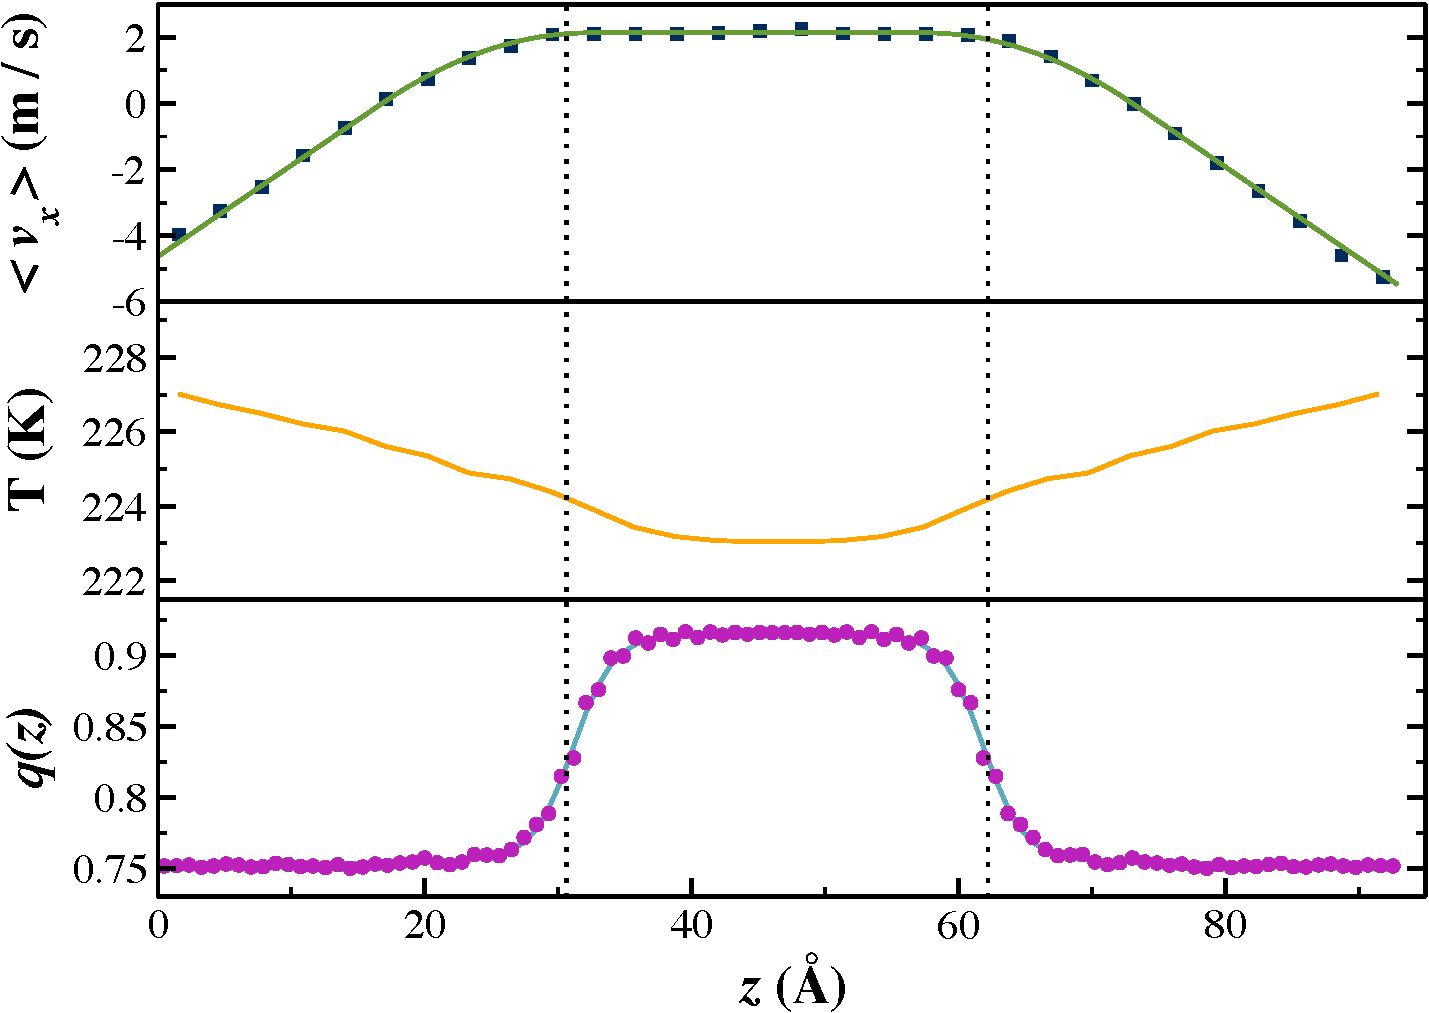
\includegraphics[width=\linewidth]{Figures/Pyr_comic_strip}
\caption{\label{fig:pyrComic} Properties of the SPC/E pyramidal
  interface being sheared through water at 7.6
  ms\textsuperscript{-1}. Lower panel: the local tetrahedral order
  parameter, $q(z)$, (circles) and the hyperbolic tangent fit
  (turquoise line).  Middle panel: the imposed thermal gradient
  required to maintain a fixed interfacial temperature of 225 K. Upper
  panel: the transverse velocity gradient (squares) that develops in
  response to an imposed momentum flux, along with the fit (green
  line). The vertical dotted lines indicate the locations of the Gibbs
  dividing surfaces of the two interfaces.}
\end{figure*}

\begin{figure*}
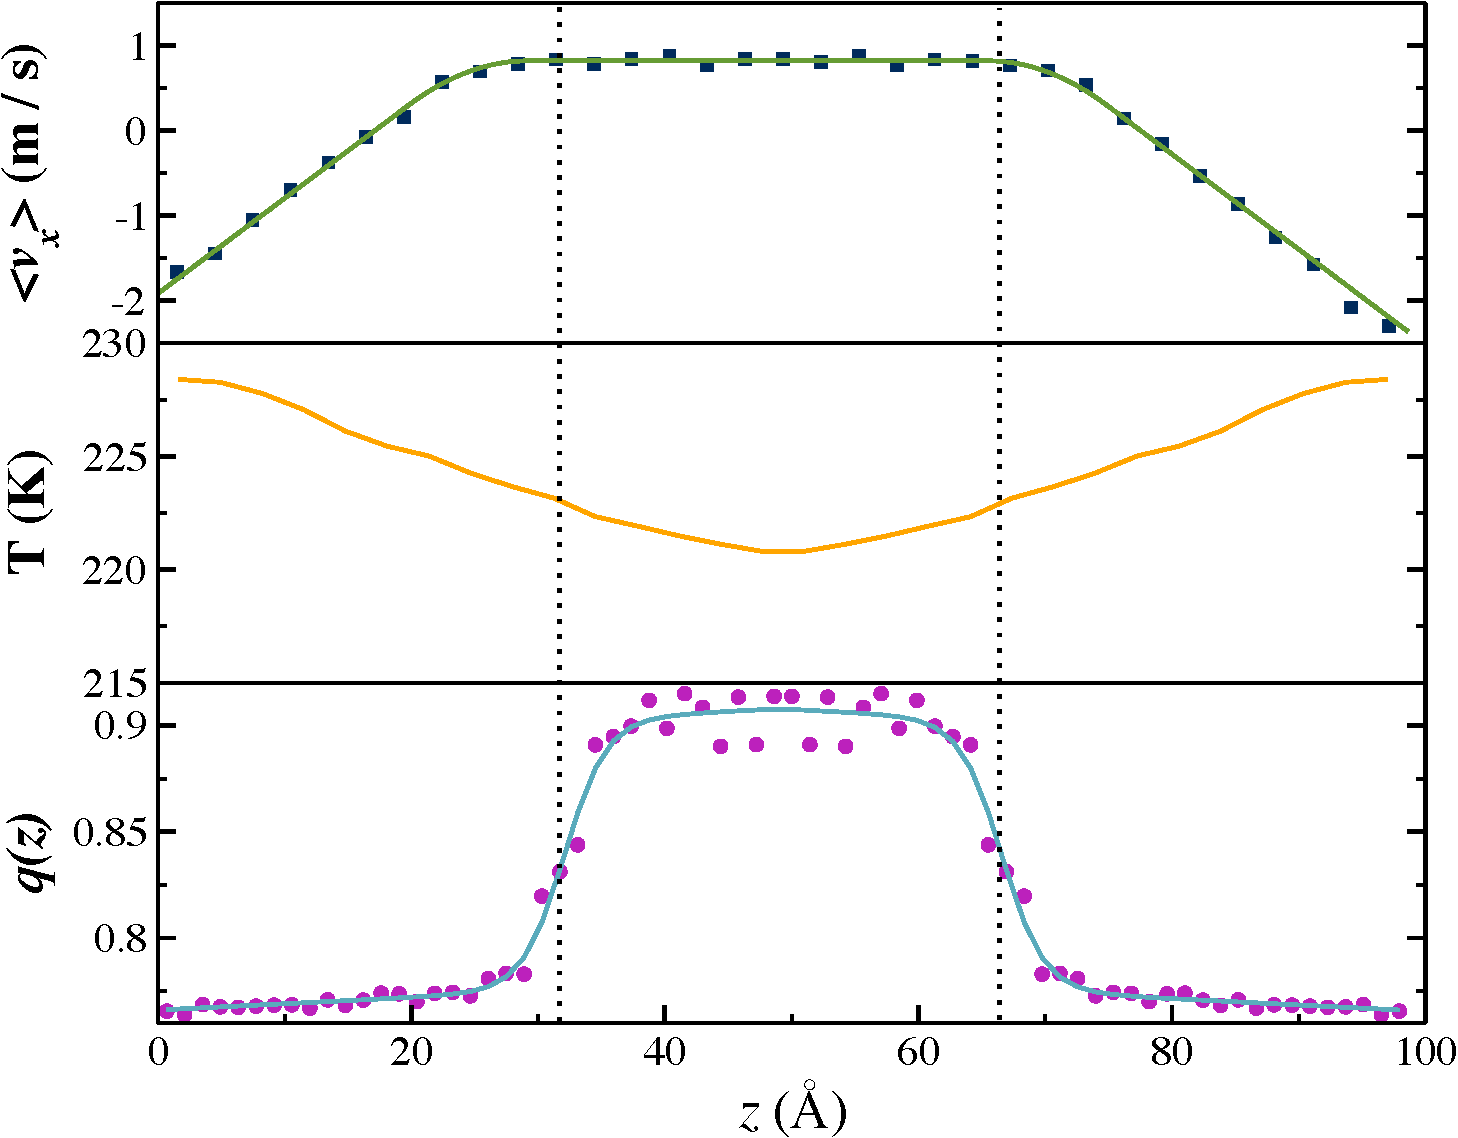
\includegraphics[width=\linewidth]{Figures/Bas_comic_strip}
\caption{\label{fig:bComic} Properties of the SPC/E basal interface being
  sheared through water at 3.2 ms\textsuperscript{-1}.  Panel
  descriptions are the same as in Figure \ref{fig:pyrComic}.}
\end{figure*}

\begin{figure*}
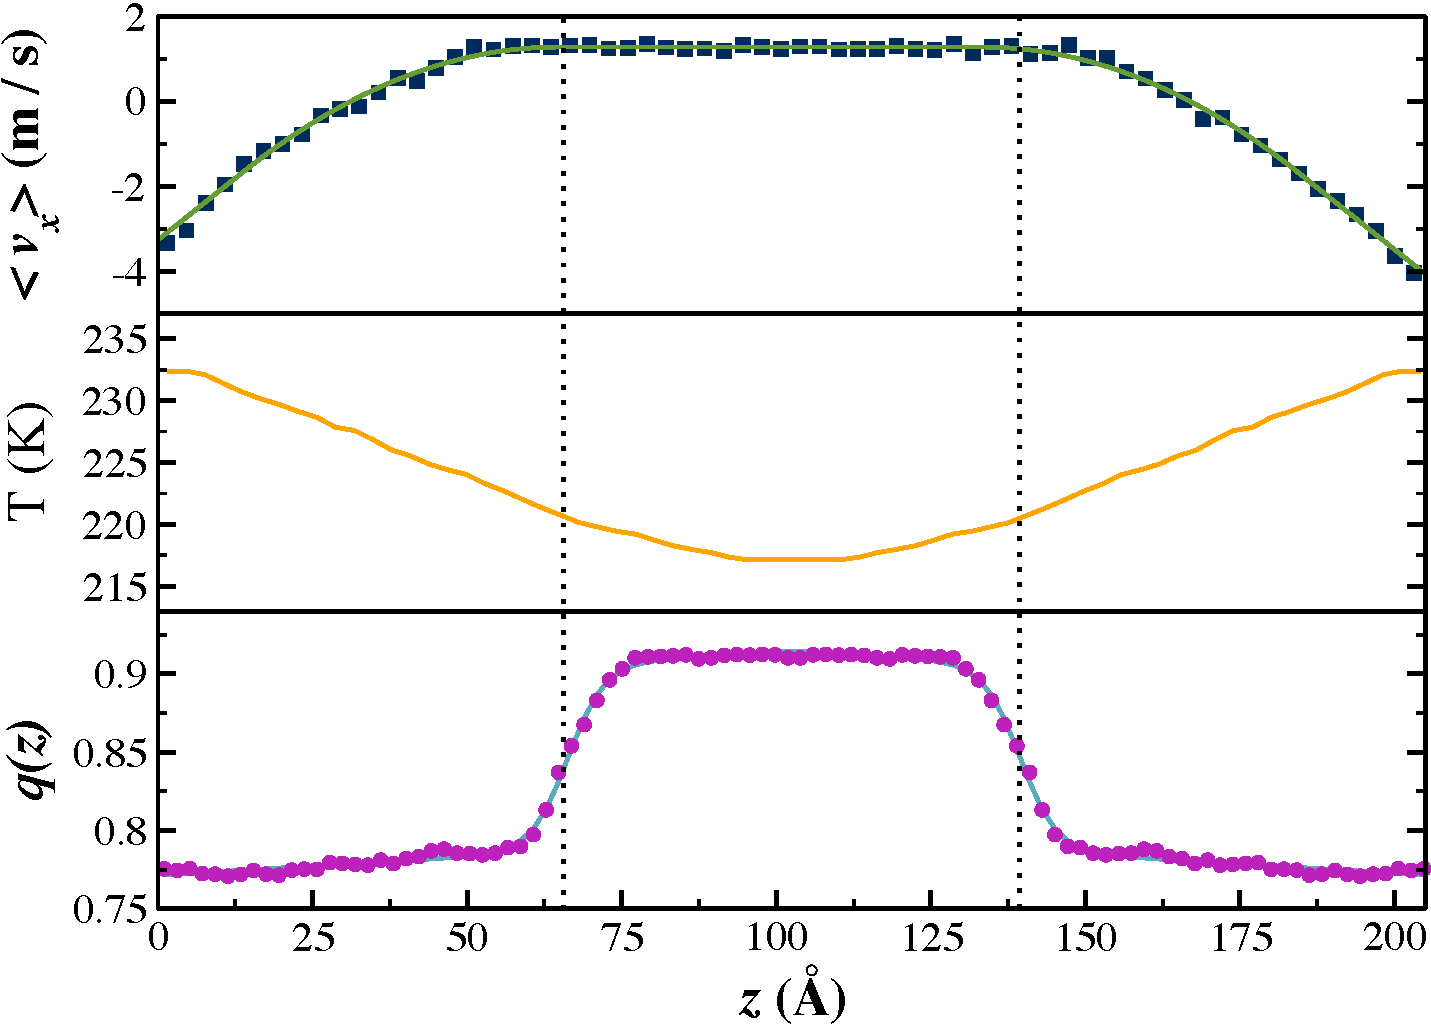
\includegraphics[width=\linewidth]{Figures/Pri_comic_strip}
\caption{\label{fig:pComic} Properties of the SPC/E prismatic interface
  being sheared through water at 6.0 ms\textsuperscript{-1}.  Panel
  descriptions are the same as in Figure \ref{fig:pyrComic}.}
\end{figure*}

\begin{figure*}
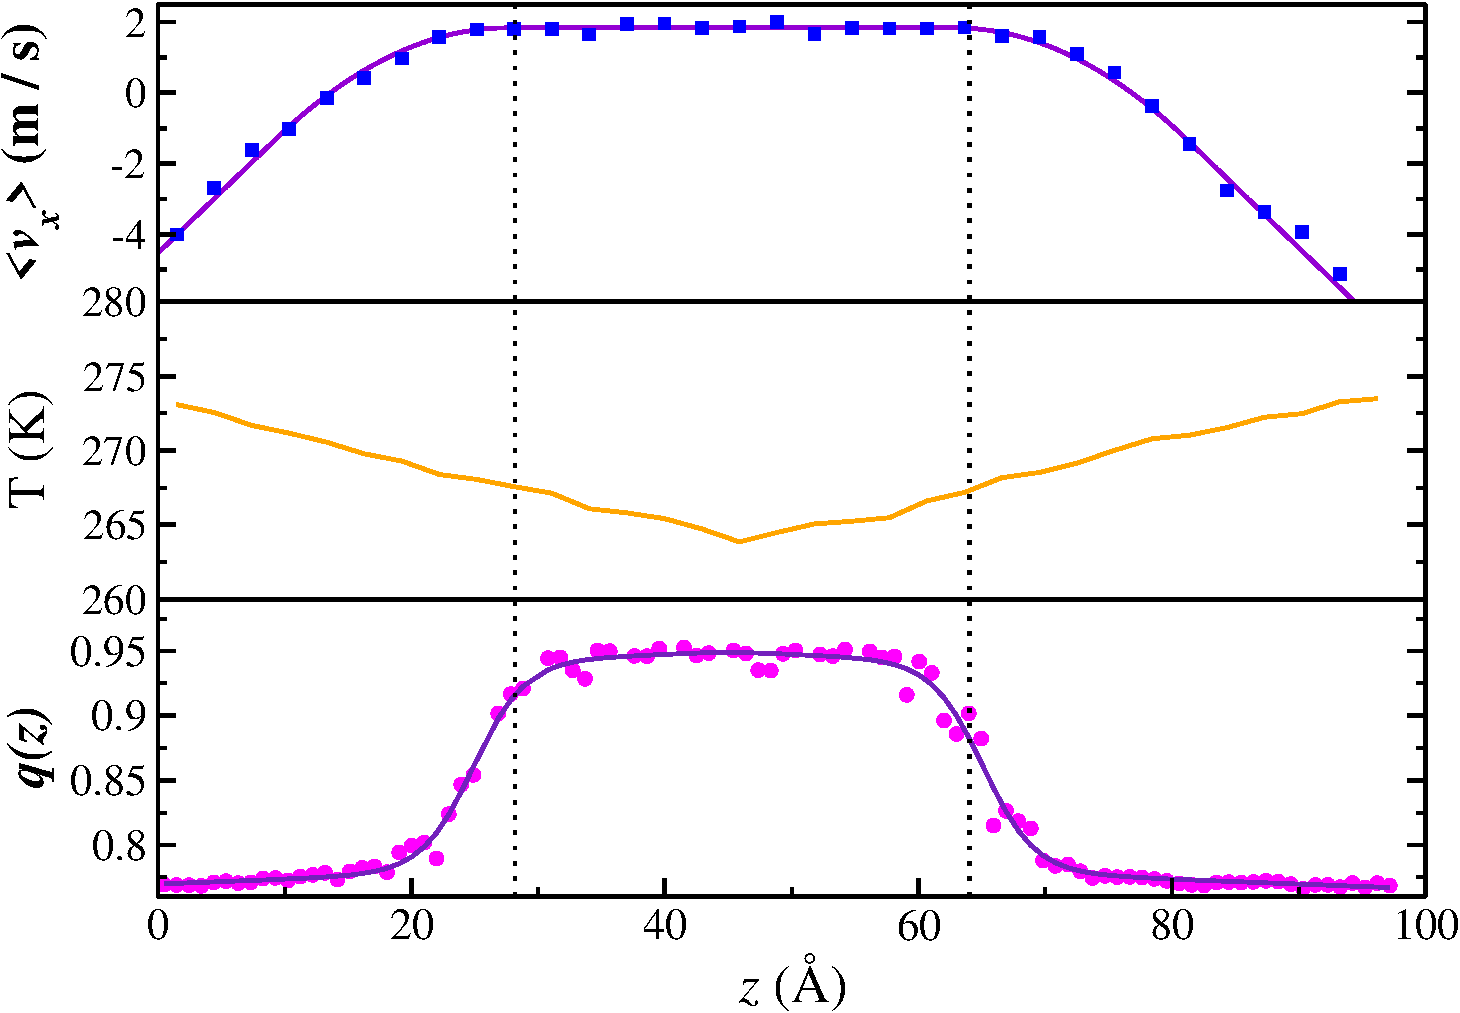
\includegraphics[width=\linewidth]{Figures/Basal_TIP4PIce_Plot}
\caption{\label{fig:tipbComic} Properties of the TIP4P/Ice basal
  interface being sheared through water at 6.1
  ms\textsuperscript{-1}. Lower panel: the local tetrahedral order
  parameter, $q(z)$, (circles) and the hyperbolic tangent fit
  (blue line).  Middle panel: the imposed thermal gradient
  required to maintain a fixed interfacial temperature of 270 K. Upper
  panel: the transverse velocity gradient (squares) that develops in
  response to an imposed momentum flux, along with the fit (purple
  line). The vertical dotted lines indicate the locations of the Gibbs
  dividing surfaces of the two interfaces.}
\end{figure*}

\begin{figure*}
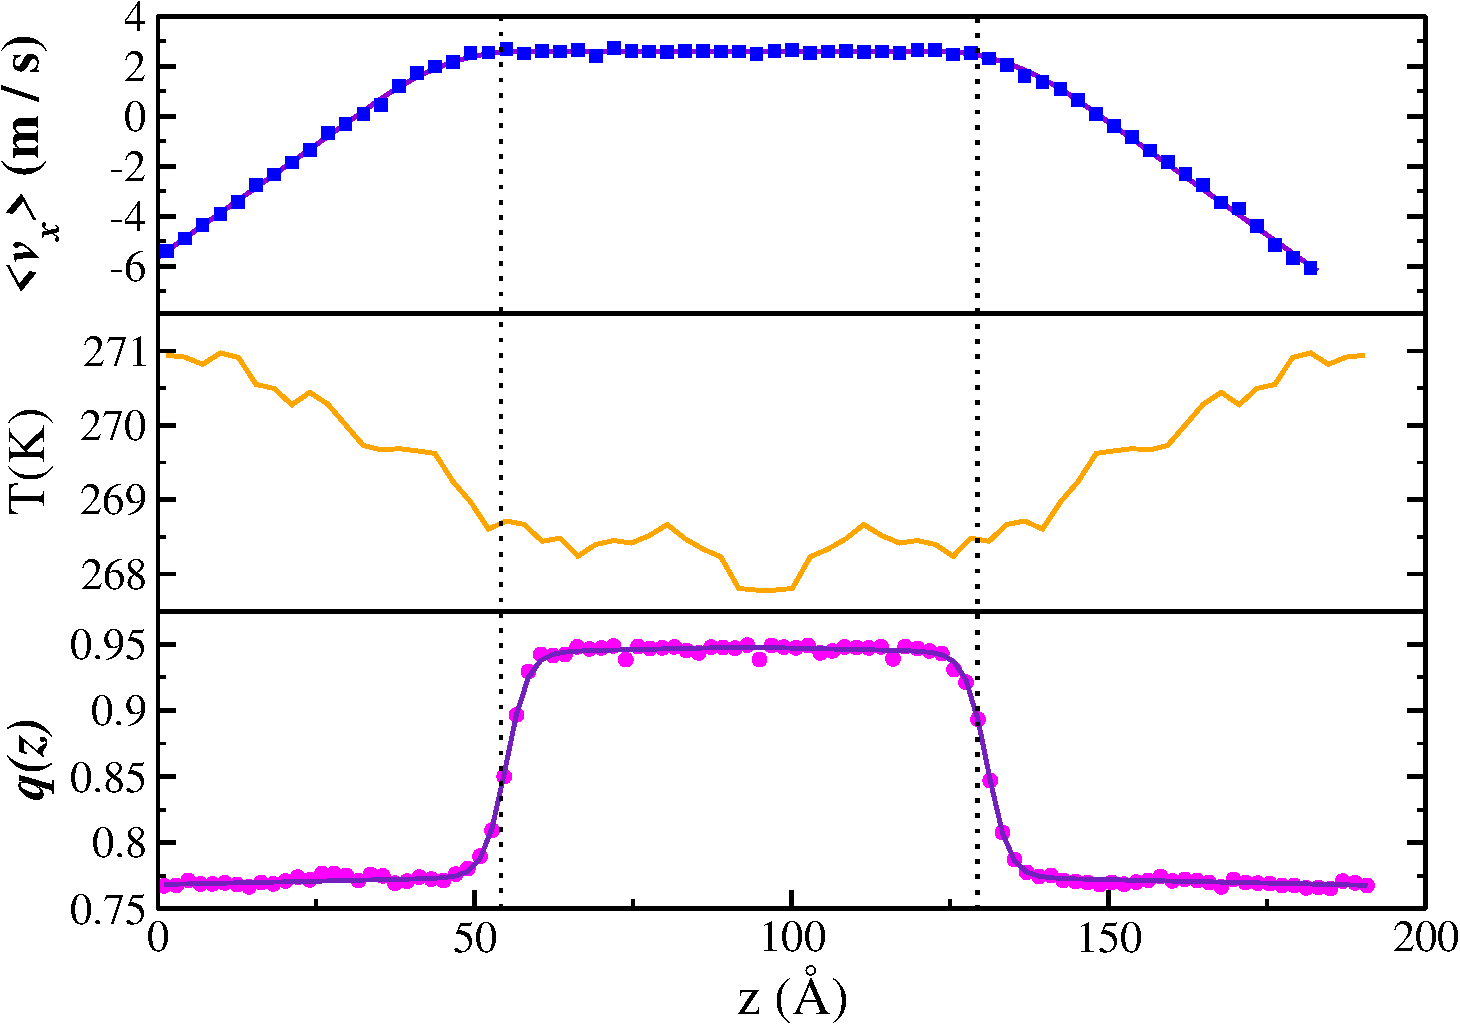
\includegraphics[width=\linewidth]{Figures/Prism_TIP4PIce_Plot}
\caption{\label{fig:tippComic} Properties of the TIP4P/Ice prismatic
  interface being sheared through water at 7.4 ms\textsuperscript{-1}.
  Panel descriptions are the same as in Figure \ref{fig:tipbComic}.}
\end{figure*}

\begin{figure*}
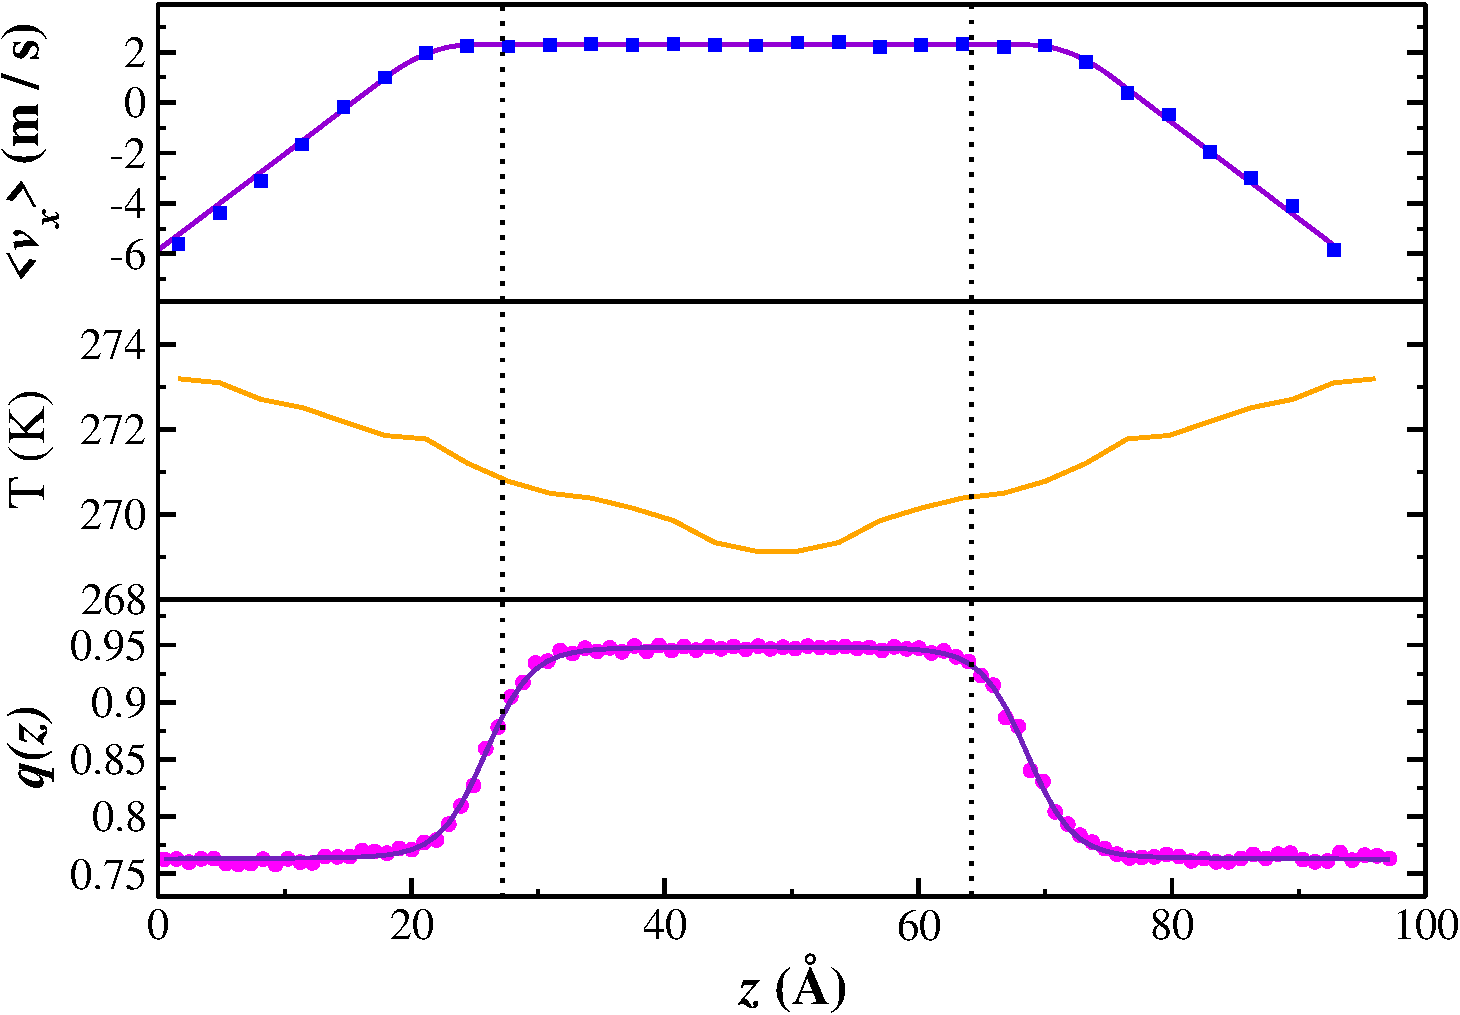
\includegraphics[width=\linewidth]{Figures/Pyra_TIP4PIce_Plot}
\caption{\label{fig:tippyComic} Properties of the TIP4P/Ice prismatic
  interface being sheared through water at 8.1 ms\textsuperscript{-1}.
  Panel descriptions are the same as in Figure \ref{fig:tipbComic}.}
\end{figure*}


\begin{figure*}
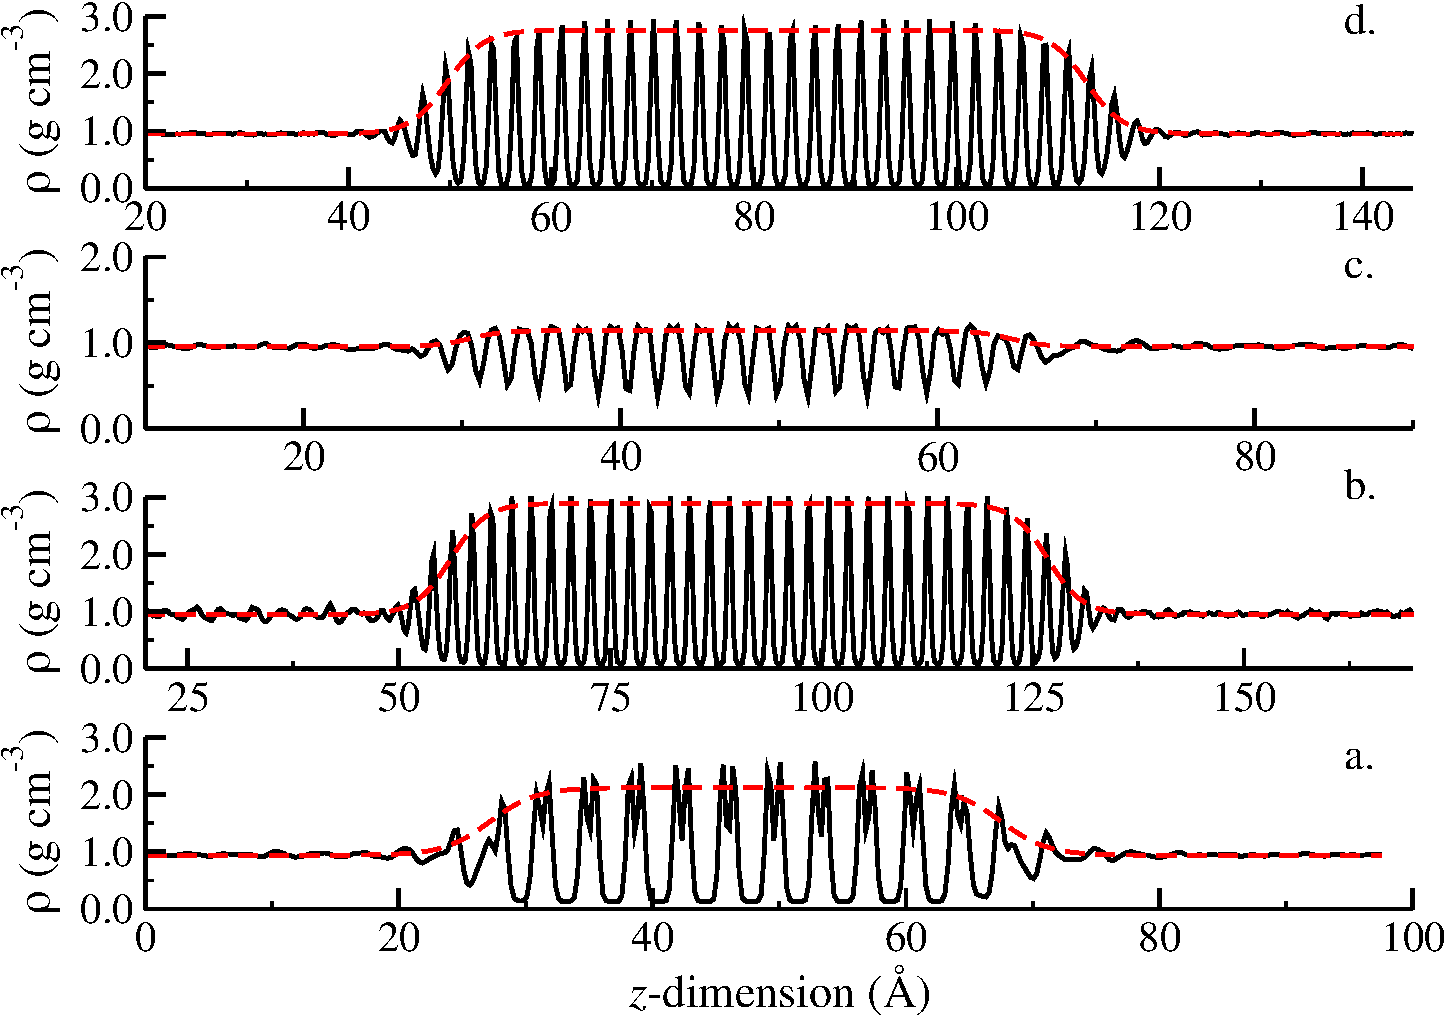
\includegraphics[width=\linewidth]{Figures/TIPtransDensity}
\caption{\label{fig:TIPtransDensity} Transverse density profiles for the
  basal (a), prismatic (b), 14\degree~pyramidal (c) and secondary prism (d)
  facets of an TIP4P-Ice ice-I$_\mathrm{h}$ / water interface (black
  lines). The prismatic and secondary prism profiles are zoomed in to
  show detail at the ice / water interface. The profiles are fit using
  Equation \eqref{rho_fit} (dashed red lines). }
\end{figure*}